\chapter{Optimization: Problem Formulation and Solution}
\label{chap:batch}

\Cref{fig:batch_opti} gives an overview on the batch optimization problem formulation.
On one hand, the real system is fed with some specific inputs and the system behaviour is measured by the available sensors.
On the other hand, virtual sensor measurements are calculated for the same inputs using a parameterized system model.
The optimization algorithm has to be designed to find the parameters that minimize the difference between the real and virtual system outputs.
\\

%For that, we formulate a cost function
%\begin{equation}
%S(\theta) = \sum_{j=1}^n ( y_j - f_j(x_j, \theta) )^2
%\end{equation}
%where $y_j$ are the measurements and $f_j(x_j, \theta)$ are the corresponding model outputs at time step $j$ and look for the parameters $\theta$ that minimize this function.
%\\

In the following section, the system model and its parameters are described.
Further, the problem is transformed into nonlinear least squares form which can be solved by the Levenberg-Marquardt algorithm. Finally, an analytical estimate for the parameter certainty is derived.

\begin{figure}[btp]
\captionsetup{width=0.9\textwidth}
\centering
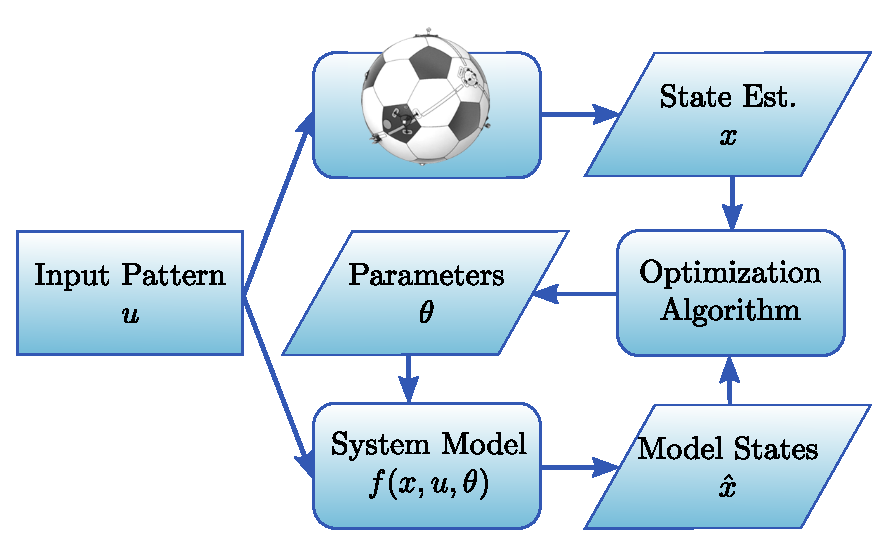
\includegraphics[width=0.7\textwidth]{images/problem_formulation.eps}
\caption{Scheme for optimization of parameterized system model.}
\label{fig:batch_opti}
\end{figure}

\section{System Model}
\label{sec:system_model}
A system model for Skye has been stated in \citep{Weichart2012} and is summarized in table \ref{tab:sys_mod}.

\begin{table}[htb!]
\centering
$\begin{array}{ll}
\toprule
\dot{\boldsymbol{\omega}}_b^b &= \mathbf{J}_b^{-1} \left( \mathbf{M}_b  - \boldsymbol{\omega}_b^b \times \mathbf{J}_b \boldsymbol{\omega}_b^b \right) \\

\dot{\mathbf{q}}_w^{b,w} &= \frac{1}{2} \mathbf{q}_w^{b,w} \otimes \left[
\begin{array}{c}
	0 \\ \boldsymbol{\omega}_b^b
\end{array} \right] \\

\dot{\mathbf{v}}_b^b &= \mathbf{\mathcal{M}}_b^{-1} \mathbf{F}_b \\

\dot{\mathbf{p}}_w^{b,w} &= \mathbf{v}_w^b \\

\bottomrule
\end{array}$
\caption{Equations of motion for Skye}
\label{tab:sys_mod}
\end{table}

It consists on the differential equations for the angular velocity $\boldsymbol{\omega}$, orientation quaternion $\mathbf{q}$, velocity $\mathbf{v}$, and position $\mathbf{p}$.
Skye is assumed as a rigid body.
Active forces and moments with respect to its center of gravity are concentrated as $\mathbf{F}$ and $\mathbf{M}$ respectively.
The total mass $\mathbf{\mathcal{M}}$ includes the rigid mass, helium mass as well as the virtual mass compensating for the inertia of the surrounding fluid.
The moment of inertia (or inertia tensor) $\mathbf{J}$ does not contain a virtual part as long as sphere like blimps are considered.
\\
For the optimization, only the angular acceleration $\boldsymbol{\alpha}$ is considered as outlined in \cref{sec:problem_evaluation}.
Subsequently, a closer look at the corresponding equation is given.

\begin{equation}
\label{eq:angular_accel}
\boldsymbol{\alpha}_b^b = \mathbf{J}_b^{-1} \left( \mathbf{M}_b  - \boldsymbol{\omega}_b^b \times \mathbf{J}_b \boldsymbol{\omega}_b^b \right)
\end{equation}

The change of angular velocity is given by the active moment $\mathbf{M}$ as well as the nutation term $\boldsymbol{\omega} \times \mathbf{J} \boldsymbol{\omega}$.
\\
The latter term influences the rotation axis such that the free body will asymptotically end in a rotation around its smallest or largest principle inertia axis.
For a homogeneous sphere, the inertia tensor is diagonal with all its diagonal elements equal and the cross product in \cref{eq:angular_accel} is therefore zero (because $\boldsymbol{\omega}$ and $\mathbf{J}\boldsymbol{\omega}$ are parallel).
As Skye itself is not as perfect symmetric as a sphere (compare \cref{sub:par_inertia}) the nutation term will be considered although it is much smaller than the active moment.
\\
The active moment $\mathbf{M}$ consists of an actuation term $\mathbf{M}^{actuation}$, a gravitation term $\mathbf{M}^{gravity}$, and an aerodynamic term $\mathbf{M}^{aero}$.

\begin{equation}
\label{eq:moments}
\mathbf{M}_b = \underbrace{\sum_{k=1}^N  \left[  \mathbf{C}_{b,m^k} \left( \mathbf{p}^{m^k,cog}_{m^k} \times \mathbf{F}^k_{m^k} \right)  \right]}_{\mathbf{M}^{actuation}}
-
\underbrace{
 \left( \mathbf{p}^{cob,cog}_b \times (\mathbf{C}_{b,w}m\mathbf{g}_w) \right)
}_{\mathbf{M}^{gravity}}
+
\mathbf{M}^{aero}
\end{equation}

For the actuation term, the moment
(cross product between position vector $\mathbf{p}^{cog,m^k}$ from COG to thruster's point of action and motor force $\mathbf{F}^k$)
is first calculated in the local motor coordinate frames $m^k$ and then transformed by the rotation matrix $\mathbf{C}_{b,m^k}$ to blimp coordinates $b$ for each motor $k=1,...,N$.

The gravity term includes the offset $\mathbf{p}^{cob,cog}$ from COG to COB and 
the gravitation force $m\mathbf{g}$. The gravitation force is only known in world coordinates $w$ and hence is transformed by the rotation matrix $\mathbf{C}_{b,w}$ from world coordinates $w$ to blimp coordinates $b$.

The aerodynamic term can be modelled as aerodynamic friction.
According to \citet{Kundu2012}, the wall shear stress is usually expressed in terms of the dimensionless skin friction coefficient $c_f$ as 
\begin{equation}
\tau_{wall} = 
\frac{1}{2} c_f \rho_{air} v^2 .
\end{equation}
The fluid velocity $v$ at the wall is composed by the angular and translational velocity of the blimp as well as the movement of the fluid itself.
For simplification, we assume the the fluid to be at rest.
The effect of the aerodynamic moment is dominated by the rotational movement of the blimp.
Because the blimp is symmetric, a pure translation would not lead to a moment.
If we assume the translational velocity much smaller than the angular velocity, it can be neglected and the wall shear stress can be integrated over the spherical hull. 
\begin{equation}
\begin{aligned}
\| \mathbf{M}^{aero} \|
&= \int_A \xi \tau_{wall} dA \\
&= \frac{1}{2} c_f \rho_{air} \int_A \xi (\xi \omega)^2 dA \\
&= \frac{1}{2} c_f \rho_{air} \omega^2 \int_{-r}^{r} (r^2-z^2)^{\frac{3}{2}} \sqrt{r^2-z^2} 2\pi dz \\
&= \frac{1}{2} c_f \rho_{air} \omega^2 \frac{32}{15} \pi r^5
 = \frac{16}{15} c_f \rho_{air} \pi r^5 \omega^2
\end{aligned}
\end{equation}

Nevertheless, this does not consider the drag of all components which are attached on the hull (e.g. actuation units or handles) which will have a significant effect on the aerodynamics.
\\

Measurements showed that the total aerodynamic drag is more than a magnitude smaller than the usual actuation moments (
$\|\mathbf{M}^{aero}(\omega = \unit[0.8]{rad/s})\| \approx \unit[0.2]{Nm} \Leftrightarrow 
\| \mathbf{M}^{actuation}_{max} \| \approx \unit[15]{Nm}$
% on the norm(omega) plot of FREE dataset (seconds 112-122) there is a decrease from 0.91 to 0.78 rad/s within 10 seconds. Hence the angular acceleration is 0.013 rad/s^2.
% alpha = J^-1 * M
% Therefore M = J*alpha = 0.13 Nm 
% We consider some margin and write ~ 0.2 Nm
). 
Therefore we neglect this term and do not further bother about its direction.
In \cref{sub:est_perf} we will show by simulation results that it is indeed valid to neglect this term.

%The position vector $\mathbf{p}^{m^k,cog}_{m^k}$ is expressed in motor coordinates too.
%As shown in \cref{sub:par_position}, this simplifies the equation a lot if the motors are placed on a sphere. The motors forces $\mathbf{F}_{m^k}$ have only nonzero components in x and y direction (see figure \ref{fig:frames})
%
%\begin{equation}
%\mathbf{F}_{m^k} = \left[ \begin{array}{c}
%F_k\cos(\varphi_k) \\
%F_k\sin(\varphi_k) \\
%0
%\end{array} \right]
%\end{equation}
%
%and the thrust $F_k$ and angle $\varphi_k$ are accurately known for the selected data samples (compare \cref{sub:data_selection}).

\section{Parameterization}
\label{sec:parameterization}
Inserting \cref{eq:moments} into \cref{eq:angular_accel}, we get the model for the angular acceleration as
\begin{align}
\lefteqn{ \mathbf{f}(\mathbf{x}, \mathbf{u}, \boldsymbol{\theta}) = {} \label{eq:sys_mod} }\\
& & {} \mathbf{J}_b^{-1} \left( 
\sum_{k=1}^N  \left[  \mathbf{C}_{b,m^k} \left( \mathbf{p}^{m^k,cog}_{m^k} \times \mathbf{F}^k_{m^k} \right)  \right]
-
\left( \mathbf{p}^{cob,cog}_b \times (\mathbf{C}_{b,w}m\mathbf{g}_w) \right)
- \boldsymbol{\omega}_b^b \times \mathbf{J}_b \boldsymbol{\omega}_b^b \right) \nonumber
\end{align}

Every variable in \cref{eq:sys_mod} must be classified as being part of the system state $\mathbf{x}$, the input $\mathbf{u}$, the parameter $\boldsymbol{\theta}$ or as a (constant) known variable\footnote{In this thesis we only use time invariant variables.
Continuous time variables can be added to batch optimization e.g. by using spline functions as shown in \citep{Furgale2012}.}.
The variables of the system model can be classified as shown in table \ref{tab:params}.

\begin{table}[htb!]
\centering
\begin{tabular}{lll}
\hline
Motor position & $\mathbf{p}^{m^k,cog}_{m^k}$ 	& param \\
Motor orientation & $\mathbf{C}_{b,m^k}$ 		& param \\
Blimp COG offset & $\mathbf{p}^{cob,cog}_b$ 	& param \\
Blimp inertia tensor & $\mathbf{J}_b$ 			& param \\
Blimp mass & $m$ 								& param \\
Actuator force & $\mathbf{F}_{m^k}^k$ 			& input \\
Blimp orientation & $\mathbf{C}_{b,w}$ 			& state \\
Blimp angular velocity & $\boldsymbol{\omega}$ 	& state \\
Gravitation & $\mathbf{g}_w$ 					& known \\
\hline
\end{tabular}
\caption{Classification of all variables of the system model equation. All variables which are subject to estimation are introduced as parameter.}
\label{tab:params}
\end{table}

In order to state a feasible problem, it must be possible to detect all parameters of the system model.
As the observability analysis in \cref{sub:observability} shows, the parameters in \cref{tab:params} are not independently observable.
Therefore it is necessary to reduce the number of parameters and replace those parameters that can easily be measured as known.
An updated classification of the variables will be shown in \cref{tab:params_updated}.
\\

There are several ways of how to represent the parameters.
We will show our choice in the sections below.

\subsection{Motor Position}
\label{sub:par_position}
In general, the motor position is a vector in the three dimensional space.
It points from the blimp's COG to the thruster's point of attack.
\begin{equation}
\mathbf{p}^{m^k,cog}
=
\left[ \begin{array}{c}
p^{m^k,cog}_1 \\
p^{m^k,cog}_2 \\
p^{m^k,cog}_3
\end{array} \right]
\in \mathbb{R}^3
\end{equation}
If we restrict the blimp hull to a perfect sphere, the ideal motor position vector space reduce to those vectors with length $r$.
The radius $r$ is the distance from the blimp's COG to the thruster's point of attack.
It is equal for all motors and the motor position expressed in the local motor frame $m^k$ (see figure \ref{fig:frames}) reduces to

\begin{equation}
\label{eq:motor_position}
\mathbf{p}^{m^k,cog}_{m^k}
=
\left[ \begin{array}{c}
0 \\
0 \\
-r
\end{array} \right]
\in \mathbb{R}^3
\end{equation}
The actual position on the hull is then simply given by the motor orientation, which is explained next.
The radius $r$ be measured by an appropriate measuring device.
As we will show in \cref{sub:observability}, a scale offset of the now 'known' motor position leads to a scale offset of the estimates about the inertia tensor $\mathbf{J}$ and COG offset $\mathbf{p}^{cob,cog}$.

\subsection{Motor Orientation}
\label{sub:par_orientation}
Since the motor thrust is known in motor coordinates $m^k$, a transformation into blimp coordinates is necessary to calculate the dynamics of the blimp.
The coordinate transformation is described by a \textit{special orthogonal group in the three dimensional space} SO(3).
The SO(3) can either be minimal represented by $3$ parameters 
(e.g. Euler angles, rotation vector, Gibbs-Rodriquez parameters) 
or nonminimal represented by $p>3$ parameters and $p-3$ constraints 
(e.g. quaternions, rotation matrix).
While minimal representations always suffer from a singularity (representation is not \textit{bijective}), nonminimal representations generally do not contain a singularity.
\\

Here we have to make the trade-off. Either we introduce one specific motor orientation which cannot be observed or we will have to solve a constraint optimization problem.
Unconstraint optimization problems are much less demanding to solve.
Therefore it is more convenient to choose a parameterization such that the motor orientation is not on the singularity.\\
If a rough estimate of the motor orientation can be made, this can be used to introduce an intermediate coordinate frame, such that the true motor orientation will not be on the singularity with very heigh probability.
Therefore, we go with minimal representation for this problem\footnote{
An alternative implementation with nonminmal representation (quaternions) using either hard or soft constraints showed worse performance than using minimal representation.
}.

Because of its computationally cheap and for optimization sufficiently smooth formula to get the rotation matrix (see \cref{eq:rod_to_C}), we use Gibbs-Rodriquez parameters $\boldsymbol{\lambda}$. Starting from rotation angle $\varphi$ and rotation axis $\mathbf{n}$, these parameters are defined as:

\begin{equation}
\boldsymbol{\lambda} = \mathbf{n} \tan(\varphi/2) 
\end{equation}

The singularity of the Gibbs-Rodriquez parameters lies at $\varphi = \pi$. 
The direction cosine transform is calculated as

\begin{equation}
\label{eq:rod_to_C}
\mathbf{C} = \mathbf{I} + \frac{2}{1+\boldsymbol{\lambda}^\top \boldsymbol{\lambda}}
\left(\boldsymbol{\lambda}^\times + \left(\boldsymbol{\lambda}^\times\right)^2\right)
\end{equation}

\subsection{Inertia Tensor}
\label{sub:par_inertia}
The inertia tensor of a rigid body is calculated as
\begin{equation}
\mathbf{J} = \int_V \rho(x,y,z) 
\left[ \begin{array}{ccc}
y^2+z^2 & - xy    & - xz \\
- xy    & z^2+x^2 & - yz \\
- xz    & - yz    & x^2+y^2
\end{array} \right] dV
\end{equation}
and is always symmetric.
In its principle frame, the off-diagonal components are zero.
We do not restrict the inertia tensor's principle frame to be aligned with the blimp frame $b$.
Therefore $\mathbf{J}_b$ is represented by six parameters\footnote{
There exist multiple variants to represent the inertia tensor. One alternative would be to decompose it into the diagonal principle form and the corresponding coordinate transformation.
}
$\boldsymbol{\vartheta} = (\vartheta_1, \hdots, \vartheta_6)'$.
\begin{equation}
\mathbf{J}_b = 
\left[ \begin{array}{ccc}
\vartheta_1 & \vartheta_4 & \vartheta_5 \\
\vartheta_4 & \vartheta_2 & \vartheta_6 \\
\vartheta_5 & \vartheta_6 & \vartheta_3
\end{array} \right]
\end{equation}


\subsection{Observability}
\label{sub:observability}
One way to analytically show observability of a system is shown by \citet{hermann1977} using Lie algebra. 
Here we do not show a proof of observability but argue which parameters are not observable and must therefore be excluded from the optimization problem.
%As we find an optimal solution for the remaining parameters, we can assume that they are observable.
\\
For convenience, we state the parameterized system model \cref{eq:sys_mod} again.
\begin{align*}
\lefteqn{ \mathbf{f}(\mathbf{x}, \mathbf{u}, \boldsymbol{\theta}) = {} }\\
& & {} \mathbf{J}_b^{-1} \left( 
\sum_{k=1}^N  \left[  \mathbf{C}_{b,m^k} \left( \mathbf{p}^{m^k,cog}_{m^k} \times \mathbf{F}^k_{m^k} \right)  \right]
-
\left( \mathbf{p}^{cob,cog}_b \times (\mathbf{C}_{b,w}m\mathbf{g}_w) \right)
- \boldsymbol{\omega}_b^b \times \mathbf{J}_b \boldsymbol{\omega}_b^b \right) \nonumber
\end{align*}

The first important observation is, that the scale of the inertia tensor $\mathbf{J}$ is only jointly observable with the scale of the motor position vectors $\mathbf{p}^{m^k,cog}$ and the COG offset $\mathbf{p}^{cob,cog}$.
If all those parameters have to be estimated, there exist infinite many solutions where the estimates are
\begin{equation}
\begin{aligned}
 \hat{\mathbf{p}}^{m^k,cog} &= \gamma \mathbf{p}^{m^k,cog} \\
 \hat{\mathbf{p}}^{cob,cog} &= \gamma \mathbf{p}^{cob,cog} \\
 \hat{\mathbf{J}}           &= \frac{1}{\gamma} \mathbf{J}
\end{aligned}
\end{equation}
for any real number $\gamma$.
The problem becomes observable, when the scale of one of those parameters is fixed, i.e. either the norm of one vector or the determinant of the tensor is assumed to be known.
Note that this scale can be chosen arbitrary with no impact on the motor orientation $\mathbf{C}_{b,m^k}$.

Because we simplified the motor position in \cref{eq:motor_position} with the scalar radius $r$, it is sufficient to assume $r$ as known to get a unique solution for all remaining parameters.
Without this simplification, a constraint optimization problem has to be solved.
\\

If one has a look at the COG offset term in \cref{eq:sys_mod}, it can be seen that the same scaling problem exists between $\mathbf{p}^{cob,cog}$ and $m$.
Here again, a wrong estimate of the fixed value $m$
would only result in a scale error of the jointly observable parameter $\mathbf{p}^{cob,cog}$ without impact on the remaining parameters\footnote{
In contrast to the COG offset $\mathbf{p}^{cob,cog}_{b}$, the mass $m$ can easily be measured on scales. Therefore we assume the scalar $m$ as known.}.
\\
The updated classification of the variables from table \ref{tab:params} is shown in table \ref{tab:params_updated}.

\begin{table}[htb!]
\centering
\begin{tabular}{lll}
\hline
Motor orientation & $\mathbf{C}_{b,m^k}$ 	& param \\
Blimp COG offset & $\mathbf{p}^{cob,cog}_b$ & param \\
Blimp inertia tensor & $\mathbf{J}_b$ 		& param \\
Actuator force & $\mathbf{F}_{m^k}^k$ 			& input \\
Blimp orientation & $\mathbf{C}_{b,w}$ 		& state \\
Blimp angular velocity & $\boldsymbol{\omega}$ & state \\
Gravitation & $\mathbf{g}_w$ 				& known \\
Blimp mass & $m$ 							& known \\
Motor POA radius & $r$ 						& known \\
\hline
\end{tabular}
\caption{Updated variable classification for the system model. Like this, all parameters are observable.}
\label{tab:params_updated}
\end{table}


\section{Nonlinear Least Squares}
As outlined above, our goal is to minimize the error between the measured and modelled angular acceleration.
For normally distributed system model errors, the maximum-likelihood estimate of the parameters is equivalent to the solution of the least squares problem \citep{Seber}.
In general, the cost function $S(\boldsymbol{\theta})$ for the ordinary nonlinear least squares problem is

\begin{equation}
S(\boldsymbol{\theta}) = \sum_{i=1}^n ( y_i - f_i(\mathbf{x}_i, \boldsymbol{\theta}) )^2
\end{equation}
which is the squared sum of the residual between observation
$y_i$
and function value
$f_i(\mathbf{x}_i, \boldsymbol{\theta})$
for
$i=1,...,n$ distinct observations.
For our problem, we group the observations to the three dimensional angular acceleration measurement vector $\mathbf{y}_j$ and the corresponding system model function\footnote{
To solve the optimization problem, we do not distinguish between inputs $\mathbf{u}$ and states $\mathbf{x}$.
In the remaining of this chapter, we will use $\mathbf{x}$ for states \textit{and} inputs for better readability and consistency with the literature.}
% XXX vilicht doch nöd als footnote? Doch! Da isch ideal als fuassnote will's a reini asichtssach isch..
$\mathbf{f}(\mathbf{x}_j, \boldsymbol{\theta})$ from \cref{eq:sys_mod}

\begin{equation}
\label{eq:cost_f_x_theta}
S(\boldsymbol{\theta}) = \sum_{j=1}^{n/3} \| \mathbf{y}_j - \mathbf{f}(\mathbf{x}_j, \boldsymbol{\theta}) \|^2
\end{equation}

and we have $n/3$ distinct angular acceleration measurements $\mathbf{y}_j$ for time steps $j=1,...,n/3$.
For being consistent with the literature, we substitute $\mathbf{x}_j$ into the function $\mathbf{f}_j(\boldsymbol{\theta})$, and use from now on
\begin{equation}
\mathbf{f}(\boldsymbol{\theta}) = \left[ \begin{array}{c}
\mathbf{f}(\mathbf{x}_1, \boldsymbol{\theta}) \\
\vdots \\
\mathbf{f}(\mathbf{x}_{n/3}, \boldsymbol{\theta})
\end{array} \right]
, \qquad
\mathbf{y} = \left[ \begin{array}{c}
\mathbf{y}_1 \\
\vdots \\
\mathbf{y}_{n/3} 
\end{array} \right]
\end{equation}

and finally get the expression for the ordinary least squares problem with the residual $\mathbf{r}$ as
\begin{equation}
\label{eq:cost_ols}
S(\boldsymbol{\theta}) = \| \mathbf{y} - \mathbf{f}(\boldsymbol{\theta}) \|^2 = \| \mathbf{r} \|^2
\end{equation}

\paragraph{Linear Regression\\}
Before we deal with the solution to the nonlinear least squares problem, we briefly review the linear case. Consider \citet[chap. 5]{Draper} for a profound treatment of linear regression.
In linear regression, the parameter vector is usually denoted by $\boldsymbol{\beta}$ and the least squares problem for a linear function 
$\mathbf{y} = \mathbf{X} \boldsymbol{\beta} + \boldsymbol{\varepsilon}$ 
with normally distributed error 
$\boldsymbol{\varepsilon} \sim \mathcal{N}(0,\mathbf{I} \sigma^2)$ 
is
\begin{equation}
S(\boldsymbol{\beta}) = \| \mathbf{y} - \mathbf{X}\boldsymbol{\beta} \|^2 = \| \mathbf{r} \|^2
\end{equation}

The least squares solution for $\boldsymbol{\beta}$ can directly be calculated as

\begin{equation}
\label{eq:linear_ls_solution}
\boldsymbol{\beta} = (\mathbf{X}' \mathbf{X})^{-1} \mathbf{X}' \mathbf{y}
\end{equation}

where
\begin{equation}
\label{eq:linear_ls_covariance}
\mathbf{V} (\boldsymbol{\beta}) = (\mathbf{X}' \mathbf{X})^{-1} {\sigma}^2
\end{equation}

is the covariance matrix of the estimates. An estimate for ${\sigma}$ is given by
\begin{equation}
\hat{\sigma}^2
= \frac{1}{n-p} (\mathbf{y} - \mathbf{X} \boldsymbol{\beta})' (\mathbf{y} - \mathbf{X} \boldsymbol{\beta})
= \frac{1}{n-p} \| \mathbf{r} \|^2
\end{equation}

\paragraph{Numerical Methods for Nonlinear Regression\\}
To find a solution for nonlinear regression, iterative schemes have to be applied \citep{Seber}.
Linear Taylor expansion of the nonlinear function
$\mathbf{f}(\boldsymbol{\theta})$ 
for 
$\boldsymbol{\theta}$
close to 
$\boldsymbol{\theta}_0$
gives
\begin{equation}
\label{eq:linearized_f}
\mathbf{f}(\boldsymbol{\theta}) \approx
\mathbf{f}(\boldsymbol{\theta}_0) + \mathbf{F}_0(\boldsymbol{\theta} - \boldsymbol{\theta}_0)
\end{equation}

where $\mathbf{F}_0$ is the Jacobian of $\mathbf{f}(\boldsymbol{\theta})$ 
evaluated at $\boldsymbol{\theta}_0$
\begin{equation}
\mathbf{F}_0 = \frac{\partial \mathbf{f}(\boldsymbol{\theta})} {\partial \boldsymbol{\theta}'} \bigg|_{\boldsymbol{\theta} = \boldsymbol{\theta}_0}
\end{equation}

%Inserting \cref{eq:linearized_f} into the cost function \cref{eq:cost_ols} yields
%\begin{align}
%S(\boldsymbol{\theta})
%&= \| \mathbf{y} - \mathbf{f}(\boldsymbol{\theta}) \|^2 \nonumber\\
%&\approx \| \mathbf{y} - \mathbf{f}(\boldsymbol{\theta}_0) - \mathbf{F}_0 (\boldsymbol{\theta} - \boldsymbol{\theta}_0) \|^2 \nonumber\\
%&= \| \mathbf{z} - \mathbf{F}_0 \boldsymbol{\beta} \|^2
%\end{align}
%where $\mathbf{z} = \mathbf{y} - \mathbf{f}(\boldsymbol{\theta}_0)$
%and $\boldsymbol{\beta} = (\boldsymbol{\theta} - \boldsymbol{\theta}_0)$.
%From linear regression, we know the least squares solution
%\begin{equation}
%\boldsymbol{\beta} = (\mathbf{F}' \mathbf{F})^{-1} \mathbf{F}' \mathbf{z}
%\end{equation}

For the residual vector $\mathbf{r}(\boldsymbol{\theta})$, we get
\begin{align}
\mathbf{r}(\boldsymbol{\theta}) 
&= \mathbf{y} - \mathbf{f}(\boldsymbol{\theta}) \nonumber\\
&\approx \mathbf{r}(\boldsymbol{\theta}) - \mathbf{F}_0(\boldsymbol{\theta} - \boldsymbol{\theta}_0)
\end{align}
and the cost function 
$S(\boldsymbol{\theta}) = \mathbf{r}(\boldsymbol{\theta})' \mathbf{r}(\boldsymbol{\theta})$
becomes

\begin{equation}
S(\boldsymbol{\theta}) \approx
\mathbf{r}(\boldsymbol{\theta}_0)' \mathbf{r}(\boldsymbol{\theta}_0) -
2 \mathbf{r}(\boldsymbol{\theta}) ' \mathbf{F}_0(\boldsymbol{\theta} - \boldsymbol{\theta}_0) + 
(\boldsymbol{\theta} - \boldsymbol{\theta}_0)'
\mathbf{F}_0' \mathbf{F}_0
(\boldsymbol{\theta} - \boldsymbol{\theta}_0)
\end{equation}
Following \citet[chap. 2]{Seber}, the cost is minimized with respect to $\boldsymbol{\theta}$ when
\begin{equation}
\boldsymbol{\theta} - \boldsymbol{\theta}_0 = 
(\mathbf{F}_0' \mathbf{F}_0)^{-1} \mathbf{F}_0' \mathbf{r}(\boldsymbol{\theta}_0)
\end{equation}

This leads to the Gauss-Newton algorithm, that is
\begin{equation}
\boldsymbol{\theta}^{i+1} =
\boldsymbol{\theta}^{i} + \boldsymbol{\delta}_i
\end{equation}

where
\begin{equation}
\label{eq:gauss_newton_step}
\boldsymbol{\delta}_i = (\mathbf{F}_i' \mathbf{F}_i)^{-1} \mathbf{F}_i' \mathbf{r}(\boldsymbol{\theta}^{i})
\end{equation}

Another iterative algorithm to find an optimal solution is the steepest-descent method.
The gradient of the cost function 
$S(\boldsymbol{\theta}) = ( \mathbf{y} - \mathbf{f}(\boldsymbol{\theta}) )'
( \mathbf{y} - \mathbf{f}(\boldsymbol{\theta}) )$
with respect to $\boldsymbol{\theta}$ is

\begin{equation}
\frac{\partial S(\boldsymbol{\theta})}{\partial \boldsymbol{\theta}} = 
- \mathbf{F} ( \mathbf{y} - \mathbf{f}(\boldsymbol{\theta}) ) = 
- \mathbf{F}  \mathbf{r}(\boldsymbol{\theta}) 
\end{equation}

From this follows the steepest-descent algorithm, that is
\begin{equation}
\boldsymbol{\theta}^{i+1} =
\boldsymbol{\theta}^{i} +
\mathbf{F}_i \mathbf{r}(\boldsymbol{\theta}^{i})
\end{equation}

\Cref{fig:steepest_descent} illustrates the working principle of the steepest-descent method for two parameters.

\begin{figure}[hbtp]
\captionsetup{width=0.9\textwidth}
\centering
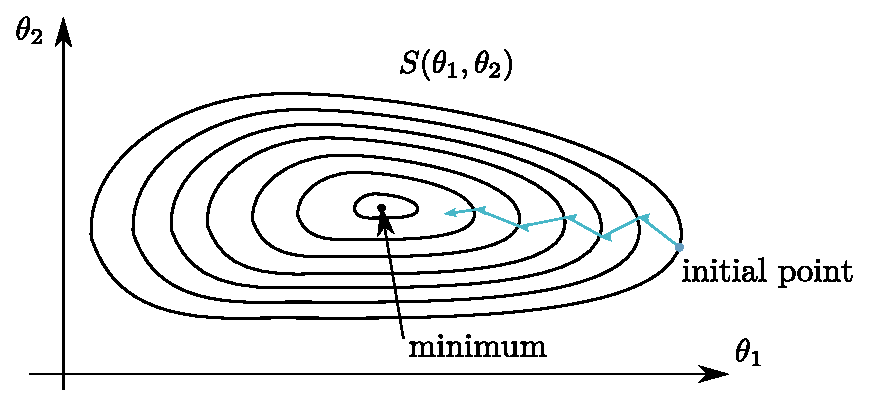
\includegraphics[width = 0.6 \textwidth]{images/steepest_descent.eps}
\caption{Starting at an initial point, the steepest-descent method iteratively proceeds into the negative direction of the gradient (down-hill) and finally converges at a (local) minimum.}
\label{fig:steepest_descent}
\end{figure}


%... Formulate minimization problem (unconstraint) as least-squares.
%... Cite \cite{Seber} (Nonlinear Regression) and maybe also \cite{Draper} (Applied Regression Analysis)

\section{Levenberg-Marquardt Algorithm}
Based on ideas by Levenberg, \citet{Marquardt1963} presented the Levenberg-Marquardt Algorithm (LMA).
As stated by \citeauthor{Marquardt1963},
steepest-descent methods (SD) have \textit{slow convergence after the first few iterations},
and Taylor series based methods, i.e. Gauss-Newton method (GN) suffer by \textit{divergence of successive iterates}.
The LMA performs an optimum interpolation between GN and SD
and is more robust than GN and has faster convergence than SD.
Using the notation introduced in the section above, LMA modifies the Gauss-Newton step \cref{eq:gauss_newton_step} to

\begin{equation}
\label{eq:lma_step}
\boldsymbol{\theta}^{i+1} =
\boldsymbol{\theta}^{i} + 
(\mathbf{F}_i' \mathbf{F}_i + \lambda_i \mathbf{I})^{-1} \mathbf{F}_i' \mathbf{r}(\boldsymbol{\theta}^{i})
\end{equation}

where $\lambda_i$ is a weighting factor between the GN and SD.
There exist several possibilities to choose $\lambda_i$.
Some implementations also use in \cref{eq:lma_step} the diagonal values of $\mathbf{F}_i' \mathbf{F}_i$ instead of $\mathbf{I}$, such that the method is not influenced by rescaling of $\boldsymbol{\theta}$.
\\

Because of its convergence rate and robustness, LMA is an appropriate algorithm for many nonlinear least square problems.
As described in \cref{chap:implementation}, we will use the \textsc{Matlab} implementation of the LMA to solve our problem.

\section{System Model Jacobian}
In this section, we will derive the Jacobian for our system model \cref{eq:sys_mod}.
In general, the Jacobian $\mathbf{F}(\boldsymbol{\theta})$ has dimension $n \times p$, where $n$ is the number of observations and $p$ is the number of parameters.
Analogue to our notation in \cref{eq:cost_f_x_theta}, we first can formulate the Jacobian $\mathbf{F}(\mathbf{x}_j, \boldsymbol{\theta}) \in \mathbb{R}^{3\times p}$ directly for the system model \cref{eq:sys_mod} and then form the Jacobian for the batch optimization as
\begin{equation}
\mathbf{F}(\boldsymbol{\theta}) = \left[ \begin{array}{c}
\mathbf{F}(\mathbf{x}_1, \boldsymbol{\theta}) \\
\vdots \\
\mathbf{F}(\mathbf{x}_{n/3}, \boldsymbol{\theta})
\end{array} \right]
\end{equation}

The $p$ columns of the Jacobian
\begin{equation}
\mathbf{F}(\mathbf{x}_j, \boldsymbol{\theta}) = 
\frac{\partial \mathbf{f}(\mathbf{x}_j, \boldsymbol{\theta})} {\partial \boldsymbol{\theta}'}
, \qquad j=1,...,\frac{n}{3}
\end{equation}

consist of the derivatives of $\mathbf{f}(\mathbf{x}_j, \boldsymbol{\theta})$
with respect to the appropriate parameter.
In the following, we use the shorthand notation $\mathbf{f}$
instead of $\mathbf{f}(\mathbf{x}_j, \boldsymbol{\theta})$.

We state again the system model from \cref{eq:sys_mod} and calculate the derivative w.r.t. the parameters as following.
\begin{equation}
\mathbf{f}
= \mathbf{J}_b^{-1} \left( 
\sum_{k=1}^N  \left[  \mathbf{C}_{b,m^k} \left( \mathbf{p}^{m^k,cog}_{m^k} \times \mathbf{F}^k_{m^k} \right)  \right]
-
\left( \mathbf{p}^{cob,cog}_b \times (\mathbf{C}_{b,w}m\mathbf{g}_w) \right)
- \boldsymbol{\omega}_b^b \times \mathbf{J}_b \boldsymbol{\omega}_b^b \right)
\end{equation}


\paragraph{Derivative w.r.t Motor Orientation\\}
As stated in \cref{sub:par_orientation}, the motor orientation is parameterized by Gibbs-Rodriquez parameters. The derivative of the direction cosine transform \cref{eq:rod_to_C} has been calculated with \textsc{Mupad} and is stated in appendix \ref{sec:app_dwrt_rodriquez}.

The derivative of the system model w.r.t. the Gibbs-Rodriquez parameters $\boldsymbol{\lambda} = (\lambda_1, \lambda_2, \lambda_3)'$ is

\begin{equation}
\frac{\partial \mathbf{f}}{\partial \lambda_i} =
\mathbf{J}_b^{-1} 
\left( \frac{\partial \mathbf{C}_{b,m^k}}{\partial \lambda_i} \right)
\left( \mathbf{p}^{m^k,cog}_{m^k} \times \mathbf{F}^k_{m^k} \right)
, \qquad i = 1,2,3
\end{equation}

\paragraph{Derivative w.r.t. Motor Position\\}
Using the rules for derivative of the cross product in appendix \ref{sec:app_d_cross_product}, the derivative of the system model w.r.t. the motor position $\mathbf{p}^{m^k,cog}_{m^k}$ is
\begin{equation}
\frac{\partial \mathbf{f}}{\partial (\mathbf{p}^{m^k,cog}_{m^k})'} =
- \mathbf{J}_b^{-1} 
\mathbf{C}_{b,m^k}
\left( \mathbf{F}^k_{m^k} \right) ^\times
, \qquad k = 1,...,N
\end{equation}

If the motor position is substituted by the radius $r$ (see \cref{eq:motor_position}), the derivative of the system model w.r.t the POA radius $r$ is simply

\begin{equation}
\frac{\partial \mathbf{f}}{\partial r} =
\mathbf{J}_b^{-1} 
\mathbf{C}_{b,m^k}
\left(
\left[ \begin{array}{c}
0 \\
0 \\
-1
\end{array} \right]
\times
\mathbf{F}^k_{m^k} \right)
, \qquad k = 1,...,N
\end{equation}

\paragraph{Derivative w.r.t. Center of Gravity\\}
The derivative of the system model w.r.t. the COG offset $\mathbf{p}^{cob,cog}_{b}$ is
\begin{equation}
\frac{\partial \mathbf{f}}{\partial (\mathbf{p}^{cob,cog}_{b})'} =
-
\mathbf{J}_b^{-1} 
\left( \mathbf{C}_{b,w} m \mathbf{g}_w \right) ^\times
\end{equation}

\paragraph{Derivative w.r.t. Inertia Tensor\\}
The derivative of the system model w.r.t. the inertia tensor parameters $\boldsymbol{\vartheta}$ is
according to the chain rule
\begin{equation}
\frac{\partial \mathbf{f}}{\partial \boldsymbol{\vartheta}'} =
-
\left(
\frac{\partial \mathbf{J}_b^{-1}}{\partial \boldsymbol{\vartheta}'}
\boldsymbol{\omega} ^\times \mathbf{J}_b \boldsymbol{\omega}
+
\mathbf{J}_b^{-1}
\boldsymbol{\omega} ^\times \frac{\partial \mathbf{J}_b}{\partial \boldsymbol{\vartheta}'} \boldsymbol{\omega}
\right)
\end{equation}
The derivative of the inverse tensor has been calculated with \textsc{Mupad}.
% and is stated in XXX APPENDIX XY.
% In XXX APPENDIX XY you can find another, analytically nicer parameterization of $\mathbf{J}$ with its derivative which has not been implemented for this work though.
\\

\section{Confidence Region}
\label{sec:confidence_region}
For having a rough idea about the certainty of the parameters found by batch optimization, the covariance matrix of the estimates for nonlinear least squares is calculated.
According to \citet[chap. 2]{Seber} the covariance can be calculated using first order Taylor series equivalent to the linear case \cref{eq:linear_ls_covariance} as

\begin{equation}
\label{eq:nlls_covariance}
\mathbf{V}(\boldsymbol{\theta}) = (\mathbf{F}(\boldsymbol{\theta})'\mathbf{F}(\boldsymbol{\theta})) ^{-1} \sigma^2
\end{equation}
where an estimate for $\sigma$ is given by
\begin{equation}
\hat{\sigma}^2 = \frac{1}{n-p} \mathbf{r}(\boldsymbol{\theta})' \mathbf{r}(\boldsymbol{\theta})
\end{equation}

To calculate the covariance of the estimated variables, we use the error propagation law as given by \citet[eq. 4.15]{Siegwart}

\begin{equation}
\label{eq:error_propagation_law}
\mathbf{V}_Y = \mathbf{G}_X \mathbf{V}_X \mathbf{G}_X'
\end{equation}
where
\begin{itemize}
\item[] $\mathbf{V}_X =$ covariance matrix of the input uncertainties;
\item[] $\mathbf{V}_Y =$ covariance matrix of the propagated uncertainties for the outputs;
\item[] $\mathbf{G}_X  $ is the Jacobian matrix of any function $\mathbf{g}$ w.r.t. $X$;
\end{itemize}

Note that \cref{eq:linear_ls_covariance} is basically the inverse formulation of \cref{eq:error_propagation_law} where $\mathbf{V}_Y = \mathbf{I} \sigma^2$.
\\

Using the estimate of the parameter covariance \cref{eq:nlls_covariance} and the error propagation law \cref{eq:error_propagation_law}, we can calculate the covariance (and hence further statistics as 95\% confidence region) of our estimates.
\\

As an example, we calculate the variance of the motor position given the variance of the Gibbs-Rodriquez parameters $\boldsymbol{\lambda}$.
The motor position, expressed in blimp coordinates $b$, is
\begin{equation}
\mathbf{p}^{m^k}_b = \mathbf{C}_{b,m^k}(\boldsymbol{\lambda}) \mathbf{p}^{m^k}_{m^k}
\end{equation}

The covariance matrix $\mathbf{V}(\boldsymbol{\lambda})$ is calculated by \cref{eq:nlls_covariance} and hence we get the error propagation by \cref{eq:error_propagation_law} as
\begin{equation}
\mathbf{V} (\mathbf{p}^{m^k}_b) = 
\left(\frac{\partial \mathbf{p}^{m^k}_b}{\partial \boldsymbol{\lambda}'}\right)
\mathbf{V}(\boldsymbol{\lambda})
\left(\frac{\partial \mathbf{p}^{m^k}_b}{\partial \boldsymbol{\lambda}'}\right)'
\end{equation}

To express the variance in the tangential reference frame $t^k$ (we will use that in \cref{chap:simulation_results}), we can apply coordinate transformation for the covariance matrix and yield
\begin{equation}
\label{eq:variance_coordinates_tangential}
\mathbf{V} (\mathbf{p}^{m^k}_{t^k}) = 
\mathbf{C}_{t^k,b}
\mathbf{V}(\boldsymbol{\lambda})
\mathbf{C}_{t^k,b}'
\end{equation}
